\section{Προθεματική Αθροιστές}
Στην ενότητα αυτή θα παρουσιαστεί μια νέα υλοποίηση αθροιστών, οι αθροιστές προθέματος,
ο οποίοι έλαβαν σημαντικό ρόλο στην επιτάχυνση καθώς και μείωση του συνολικού εμβαδού 
των αθροιστών. 





\subsection{Πρόβλημα προθέματος}

Ένα prefix problem ή πρόβλημα προθέματος 
ορίζεται από n εξόδους y ( $y_{n-1},y_{n-2}, ... ,y_0 $ ) , n εισόδους x ( $x_{n-1},x_{n-1}, ... ,x_0 $ ) και τον τελεστή $\circledast$ .
Κάθε έξοδος y υπολογίζεται με τον παρακάτω τρόπο :
\begin{equation}
\begin{split}
y_0 &= x_0\\
y_1 &= x_1 \circledast x_0\\
y_2 &= x_2 \circledast x_1 \circledast x_0\\
&...\\
y_{n-1} &= x_{n-1} \circledast x_{n-2} \circledast ... \circledast x_{1} \circledast x_0\\
\end{split}
\end{equation}

Επίσης μπορούμε να το εκφράσουμε και αναδρομικά :
\begin{equation}
\begin{split}
y_0 &= x_0\\
y_{i} &= x_{i} \circledast y_{i-1}\\
\end{split}
\end{equation}

Ένα απλό παράδειγμα προβλημάτων που αντιμετωπίζονται ως προβλήματα προθέματος είναι 
η πρόσθεση πολλών αριθμών. Έστω πως έχουμε ένα σύνολο μεγέθους n από αριθμούς 
$(x_{n-1},x_{n-2}, ... ,x_1,x_0)$, σύμφωνα με τον ορισμό που δόθηκε παραπάνω
χρειαζόμαστε ένα ακόμα σύνολο ίδιου μεγέθους $(y_{n-1},y_{n-2}, ... ,y_1,y_0)$ 
όπου κάθε στοιχείο του συνόλου αυτού υπολογίζεται αναδρομικά
\begin{equation*}
\begin{split}
y_0 &= x_0\\
y_{i} &= x_{i} + y_{i-1}\\
\end{split}
\end{equation*}
και το τελικό αποτέλεσμα είναι καταχωρημένο στο $y_n-1$.

Το πρόβλημα υπολογισμού κρατουμένου μπορούμε να το μετατρέψουμε σε
prefix problem δημιουργώντας το ζεύγος $(G,P)$ και αναθέτοντας στον τελεστή
$\circledast$ την παρακάτω λειτουργιά :
\begin{equation}
\begin{split}
(g_i,p_i) \circledast (g_k,p_k) &= (g_i + p_ig_k , p_ip_k)\\
(G_i,P_i) \circledast (G_k,P_k) &= (G_i + P_iG_k , P_iP_k)
\end{split}
\end{equation}

Με αυτόν τον τρόπο μπορούμε να υπολογίσουμε κάθε ενδιάμεσο κρατούμενο $c_i$
καθώς και το κρατούμενο εξόδου $c_n$ για έναν αθροιστή των n-bits όπου $c_i = G_i$
και για $n \geq i \geq 0$ έχουμε 
\begin{equation}
\equationame{Αλγεβρικός ορισμός των $(G_i,P_i)$}
\begin{split}
(G_0,P_0) &= (g_0,p_0)\\
(G_i,P_i) &= (g_i,p_i) \circledast (G_{i-1},P_{i-1})
\end{split}
\end{equation}
Η απόδειξη :
Εφόσον δεν υπάρχει κρατούμενο εισόδου ($c_{in} = c_{-1} = 0$) έχουμε 
\begin{equation*}
\begin{split}
    c_0 &= g_0 + p_0c_{-1} \\
    c_0 &= g_0 \\
    c_0 &= G_0
\end{split}
\end{equation*}
έστι το αποτέλεσμα ισχύει για $i-1$ \\
Αν $i>0$ και $c_{i-1} = G_{i-1}$ τοτε
\begin{equation*}
\begin{split} 
    (G_i,P_i)   &= (g_i,p_i) \circledast (G_{i-1},P_{i-1}) \\
                &= (g_i,p_i) \circledast (c_{i-1},P_{i-1}) \\
                &= (g_i + p_ic_{i-1} , p_iP_{i-1}) \\
            G_i &= g_i + p_ic_{i-1} \\
            G_i &= c_i
\end{split}
\end{equation*}
Επίσης ο τελεστής $\circledast$ έχει προσεταιριστική ιδιότητα 
\begin{equation*}
\begin{split} 
    (g_i,p_i)\circledast(g_j,p_j)\circledast(g_k,p_k) &= [g_i + p_ig_j,p_ip_j]\circledast(g_k,p_k) \\
    &= (g_i,p_i)\circledast[g_j + p_jg_k,p_jp_k]\\
    &= ( g_i + p_ig_j + p_ip_jg_k , p_ip_jp_k )
\end{split}
\end{equation*}

Παρακάτω παρουσιάζεται ένα γράφημα-δέντρο ( Εικόνα \ref{Serial-PrefixTree} ) 
ενός απλού διάδοσης κρατουμένου αθροιστή σε αναγόμενο σε πρόβλημα προθέματος.\\ 
\begin{figure}[H]
\centering
% 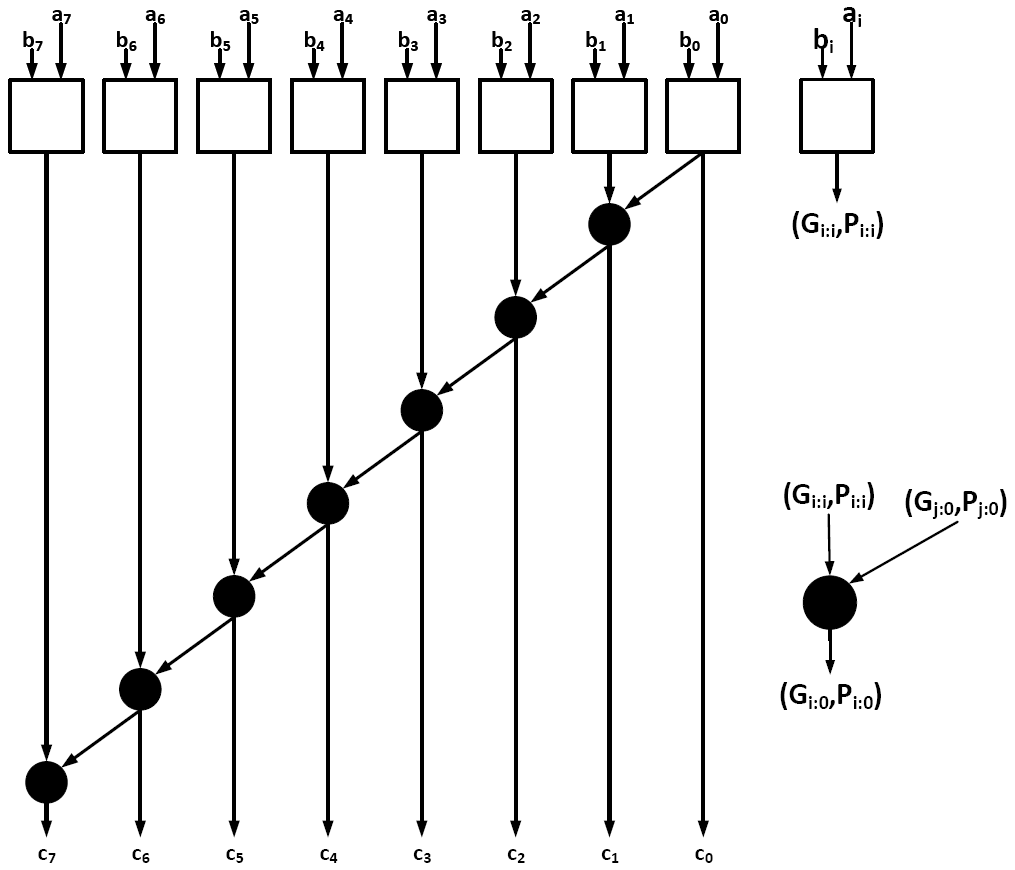
\includegraphics[width=\textwidth]{Serial-Prefix.png}
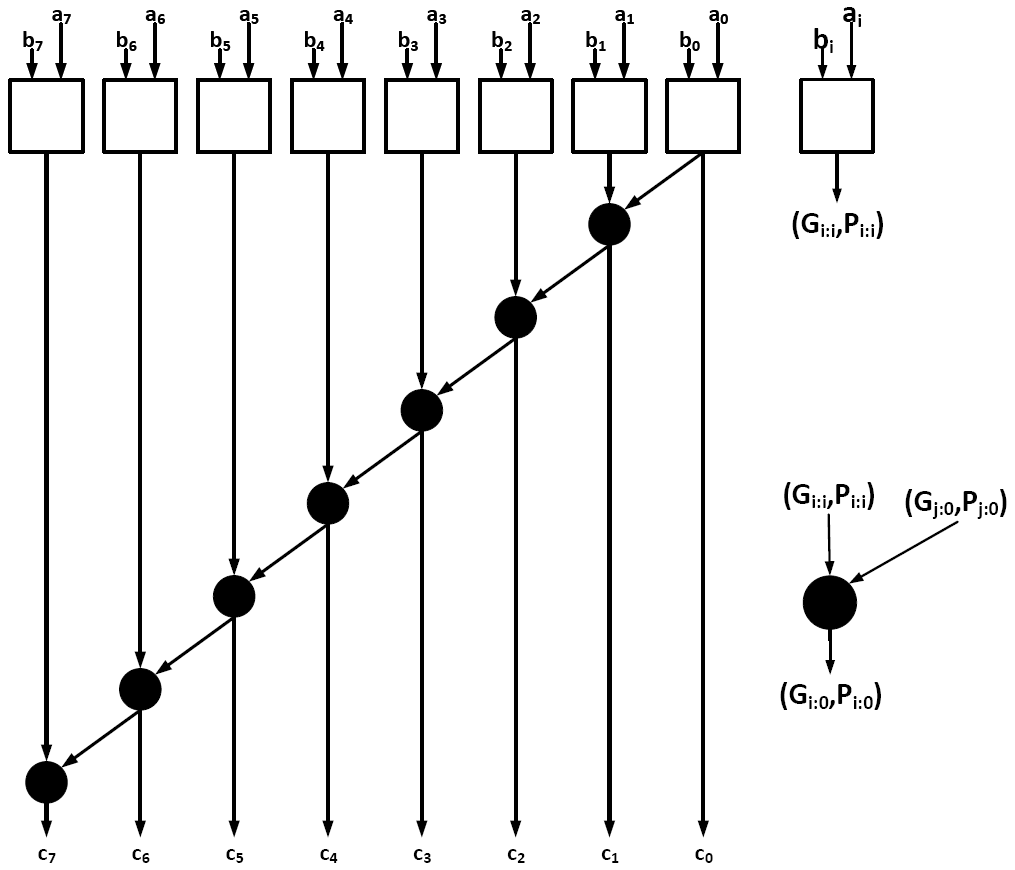
\includegraphics[scale=0.4]{Serial-Prefix.png}
\caption{Serial-Prefix Tree Adder}
\label{Serial-PrefixTree}
\end{figure}
Σε κάθε μαύρο κόμβο ουσιαστικά υλοποιείται η λογική συνάρτηση του τελεστή $\circledast$
που παρουσιάστηκε προηγουμένως. Ο παραπάνω αθροιστής υλοποιεί τον προθεματικό αλγόριθμο
σειριακά με αποτέλεσμα να είναι πολύ αργό το μοντέλο αλλά να καταλαμβάνει μικρότερο εμβαδόν
από άλλες τοπολογίες αθροιστών προθέματος που θα παρουσιαστούν στην συνέχεια.














\subsection{Παράλληλοι Προθεματικοί Αθροιστές}
Η διάταξη που παρουσιάστηκε στην εικόνα \ref{Serial-PrefixTree} έχει την δομή 
του απλού αθροιστή διάδοσης κρατουμένου εκφρασμένο σε προθεματική μορφή. Ο προθεματικός
όμως υπολογισμός κρατουμένων μπορεί να υπολογιστεί παράλληλα, αποτελώντας την προθεματική 
έκφραση ως κινητήριο παράγοντα διάφορων παράλληλων αρχιτεκτονικών που προτάθηκαν.
Μερικές σημαντικές αρχιτεκτονικές διατυπώνονται στις επόμενες παραγράφους με σύντομη
περιγραφή.




\subsection{Δέντρα-Δομές Προθεμάτων}

\begin{figure}[H]
    \centering
    %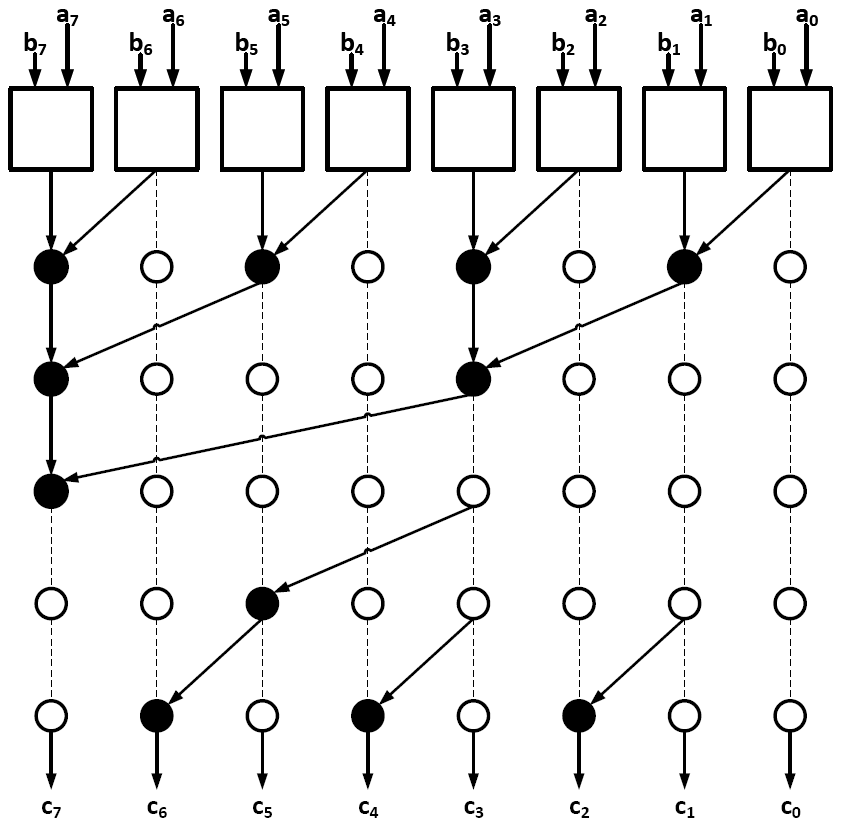
\includegraphics[width=\textwidth]{Brent_Kung_Prefix.png}
    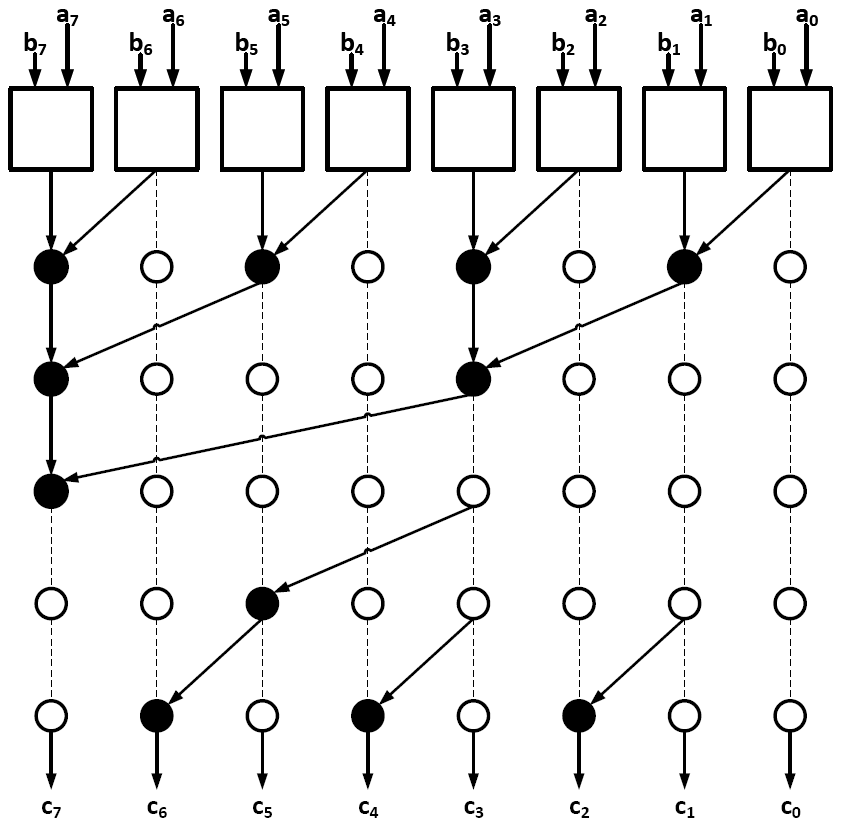
\includegraphics[scale=0.45]{Brent_Kung_Prefix.png}
    \caption{Brent-Kung Prefix Tree Adder}
    \label{BrentKungTree}
\end{figure}


% \subsubsection{Ladner-Fischer Adder}
% \textcolor{red}{Ανελυσε Ladner-Fischer}
\begin{figure}[H]
    \centering
    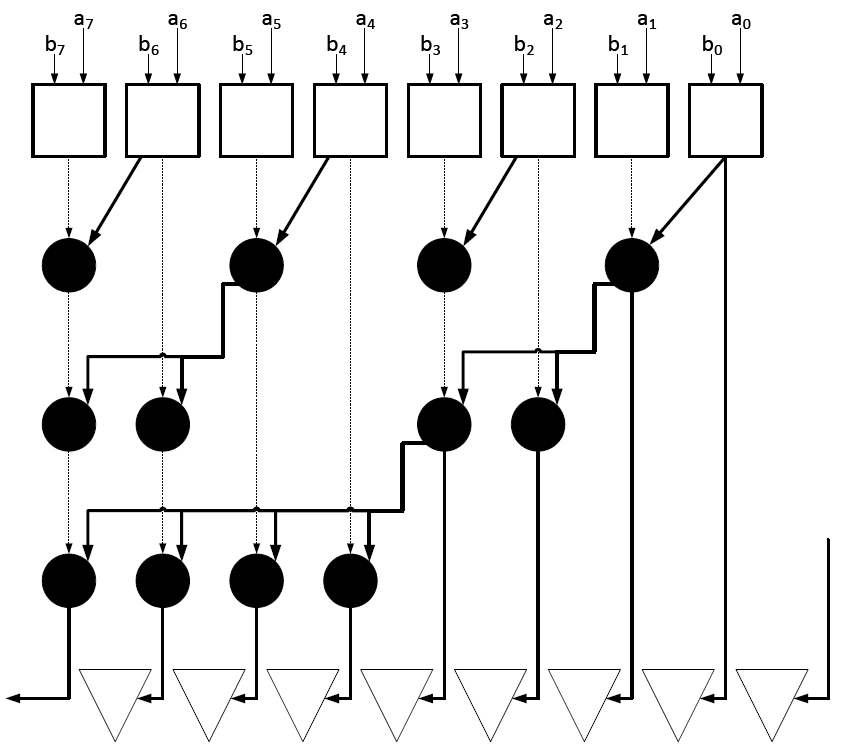
\includegraphics[scale=0.4]{Ladner-Fischer.png}
    \caption{J. Sklansky Prefix Tree Adder}
    \label{Ladner-FischerTree}
\end{figure}

\textcolor{red}{
R.P. Brent and H.T. Kung, A Regular Layout for Parallel
Adders,º IEEE Trans. Computers, vol. 31, no. 3, pp. 260-264, Mar.
1982.
\\\\
P.M. Kogge and H.S. Stone, A Parallel Algorithm for the Efficient
Solution of a General Class of Recurrence Equations, IEEE Trans.
Computers, vol. 22, no. 8, pp. 783-791, Aug. 1973.
\\\\
J. Sklansky, Conditional Sum Addition Logic, IRE Trans.
Electronic Computers, vol. 9, no. 6, pp. 226-231, June 1960.
}













\subsection{Αραίωση των Δέντρων}
Οι δομές που περιγράφηκαν για την παραλληλοποίηση του υπολογισμού των κρατουμένων 
είναι αρκετά πυκνά όσο αφορά τους μαύρους κόμβου, το οποίο συνεπάγει το ότι 
απαιτείται αρκετή ενέργεια και εμβαδόν. Με σκοπό την αραίωση (sparseness), 
είναι δυνατό να υπολογίζονται λιγότερα κρατούμενα από τα ενδιάμεσα στάδια,
δηλαδή το δέντρο, και υπολογίζοντας τα υπόλοιπα με διάδοση.

Για παράδειγμα υπολογίζοντας το κρατούμενο που παράγεται από το τρίτο έως το 
μηδενικό δυαδικό ψηφίο, δηλαδή το $G_{3:0}$ και εισάγωντας στο στο κρατούμενο 
εισόδου ενός αθροιστή επιλογής κρατουμένου (CSA) των τεσσάρων δυαδικών ψηφίων 
με είσοδο τα δυαδικά ψηφία $7:0$ \cite{Sparseness_ling}.
\\\\ 
Sparsness-2
\begin{equation*}
    \begin{split}
        sum_i &= x_i \oplus G_{i-1:0}\\
        sum_{i+1} &= x_{i+1} \oplus G_{i:0}\\
        &= x_{i+1} \oplus (g_i + p_i*G_{i-1:0})\\
    \end{split} 
\end{equation*}
Sparsness-4
\begin{equation*}
    \begin{split}
        sum_i &= x_i \oplus G_{i-1:0}\\
        sum_{i+1} &= x_{i+1} \oplus G_{i:0}\\
        &= x_{i+1} \oplus (g_i + p_i*G_{i-1:0})\\
        sum_{i+2} &= x_{i+2} \oplus G_{i+1:0}\\
        &= x_{i+2} \oplus (g_{i+1} + p_{i+1}g_i + p_{i+1}p_iG_{i-1:0})\\
        sum_{i+3} &= x_{i+3} \oplus G_{i+2:0}\\
        &= x_{i+3} \oplus (g_{i+2} + p_{i+2}g_{i+1} + p_{i+2}p_{i+1}g_i + p_{i+2}p_{i+1}p_iG_{i-1:0})\\
    \end{split} 
\end{equation*}



\subsection{Προθεματικός αθροιστής με κρατούμενο εισόδου}
Οι αθροιστές προθέματος που παρουσιάστηκαν παραπάνω αναπτύχθηκαν με την αρχική
υπόθεση έλλειψης κρατουμένου εισόδου ή $c_{in} = 0$. Ενσωματώνοντας στους παραπάνω 
αθροιστές την επιλογή κρατουμένου εισόδου $c_{in}$, το οποίο ταυτίζεται με το σήμα $c_{-1}$
, ορίζεται το αντίστοιχο ζεύγος σημάτων $(G'_i,P'_i)$, όπου είναι το Grou Generate και 
Group Propagate αντίστοιχα με την διαφορά πως συμπεριλαμβάνουν και το κρατούμενο εισόδου.
Ακολουθεί ο αλγεβρικός ορισμός των σημάτων $G'_i$ και $P'_i$ ( εξίσωση \ref{eq:GP_with_carry_in} )
\begin{equation}
    \equationame{Αλγεβρικός ορισμός των $(G'_i,P'_i)$}
    \label{eq:GP_with_carry_in}
    (G'_i,P'_i) = 
    \begin{cases}
        (g_0 + p_0*c_{-1} , p_0)   , & i = 0\\
        (g_i,p_i)\circledast (G'_{i-1},P'_{i-1}) , & 1 \leq i \leq n-1
    \end{cases}
\end{equation}
Επίσης, στην περίπτωση που συνυπολογίζεται και το κρατούμενο εισόδου, προφανώς ισχύει και 
$c_i = G'_i$. Για την ανάκτηση των $(G'_i,P'_i)$ χρησιμοποιείται ο παρακάτω τύπος:
\begin{equation}
    \label{eq:G'P'_From_GP}
    \equationame{Ανάκτηση των $(G'_i,P'_i)$ από $(G_i,P_i)$}
    (G'_i,P'_i) = (G_i + P_i*c_{-1} , P_i)
\end{equation}
το οποίο αποδεικνύεται επίσης επαγωγικά στο $i$. Για $i=0$ ισχύει :
\begin{equation*}
    (G'_0,P'_0) = (g_0 + p_0*c_{-1} , p_0) =  (G_0 + P_0*c_{-1} , P_0)
\end{equation*}
Υποθέτοντας πως η σχέση ισχύει και για $i=k-1$, δηλαδή
\begin{equation*}
    (G'_{k-1},P'_{k-1}) = (G_{k-1} + P_{k-1}*c_{-1} , P_{k-1})
\end{equation*}
Τότε για $i=k$ :
\begin{equation*}
    \begin{split}
        (G'_k,P'_k) &= (g_k,p_k) \circledast (G'_{k-1},P'_{k-1})\\
                    &= (g_k,p_k) \circledast (G_{k-1} + P_{k-1}*c_{-1} , P_{k-1}) \\
                    &= ( g_k + p_k*(G_{k-1} + P_{k-1}*c_{-1}) , p_k*P_{k-1} ) \\
                    &= \big( (g_k + p_kG_{k-1}) + p_kP_{k-1}c_{-1} , P_k  \big) \\
                    &= ( G_k + P_k*c_{-1} , P_k )
    \end{split}
\end{equation*}
\\
Όσο αφορά την τροποποίηση των γραφημάτων για τον συνυπολογισμό κρατουμένου εισόδου
είναι δυνατό να κρατηθεί ανέπαφη η δομή υπολογίζοντας τα Group Generate και Group Propagate 
$(G_i,P_i)$ χωρίς το κρατούμενο εισόδου  και στο τέλος προστίθεται ένα ακόμα επίπεδο
για κάθε δυαδικό ψηφίο $i$ που υλοποιείται η λογική $G_ι + P_ι*c_{-1}$.
\\\\
\textcolor{red}{[Βάλε σχήμα που δείχνει το extra επίπεδο]}
\\\\
\textcolor{red}{[Βάλε και σχήμα με Kogge-Stone δομή με $c_{in}$]}
\\\\


